\section{Interplay of Redundant Samples and Weights}
\label{sec:poly}
We explore the interplay between redundant weights and samples by investigating their impact on weight pruning and coreset selection. 
In order to provide mathematically transparent analysis, we apply standard pruning and coreset selection techniques to polynomial interpolation.

\paragraph{Impact of redundant samples on weight pruning.} We study this impact on the polynomial interpolation task with a classic example  
Runge's function \( f(x) = \frac{1}{1 + 25x^2}, \, x \in [-1, 1] \)~\cite{runge1901empirische}, which is smooth and has derivatives of all orders, as shown by the {\color{blue}blue curve} in Fig.~\ref{fig:fit_10} and~\ref{fig:fit_5} (see appendix for results on other functions).
Our dataset comprises 10 points sampled from the function: 5 are clean data points (which form the coreset), and the other 5 are noisy points, generated by adding Gaussian noise with a magnitude of 0.1. Using the least squares method, we fitted a \(10^{\text{th}}\)-degree polynomial to two datasets separately: the full dataset of 10 points and the 5-point coreset. Following the standard weight pruning techniques~\cite{han2016deep}, we pruned the three smallest coefficients (in magnitude) by setting them to zero while retaining the remaining coefficients. 
Our findings indicate that an increased number of data points, especially those containing noise, renders pruning more challenging. This is evidenced by the higher loss observed ({\color{orange}yellow curve} in Fig.~\ref{fig:fit_10}) after pruning, which suggests that coreset selection can enhance the effectiveness of pruning in scenarios involving redundant samples.

\paragraph{Impact of redundant weights on coreset selection.}
The goal of coreset selection is to identify a small subset of training data that approximates the objective function of the entire dataset throughout the parameter space. A typical formulation is constructed on function approximation, which involves finding a small subset \( \hat{\mathcal{D}} \) from the training dataset \( \mathcal{D} \) such that:
\begin{align}
   \frac{|\mathcal{L}(\boldsymbol{\theta}) - \hat{\mathcal{L}}(\boldsymbol{\theta})|}{\mathcal{L}(\boldsymbol{\theta})} \leq \epsilon , ~\text{for any } \boldsymbol{\theta} \in \mathbb{R}^p, \label{eq:epsilon}
\end{align}
where \( \mathcal{L}(\boldsymbol{\theta}) = \frac{1}{|\mathcal{D}|} \sum_{i \in \mathcal{D}} \ell(\boldsymbol{\theta}; x_i, y_i) \) is the objective function on the full dataset, and \( \hat{\mathcal{L}}(\boldsymbol{\theta}) = \frac{1}{|\hat{\mathcal{D}}|} \sum_{i \in \hat{\mathcal{D}}} \ell(\boldsymbol{\theta}; x_i, y_i) \) is the objective function on the selected subset \( \hat{\mathcal{D}} \). Here, \( \epsilon \) is a small number that controls the approximation error. When \( \epsilon \) is sufficiently small, the model performance learned from \( \hat{\mathcal{L}} \) can be comparable to that learned from \( \mathcal{L} \). In this context, 
\begin{align}
   \mathcal{I}(\mathcal{D}, \hat{\mathcal{D}}) = \sup_{\boldsymbol{\theta}}\frac{|\mathcal{L}(\boldsymbol{\theta}) - \hat{\mathcal{L}}(\boldsymbol{\theta})|}{\mathcal{L}(\boldsymbol{\theta})}, \label{eq:idd}
\end{align}
can be used to evaluate the difficulty of coreset selection. The reason is that given two fixed datasets $\mathcal{D}$ and $\hat{\mathcal{D}}$, if $\mathcal{I}(\mathcal{D}, \hat{\mathcal{D}}) $ for network $f_1(\cdot, \boldsymbol{\theta})$ is larger than network $f_2(\cdot, \boldsymbol{\theta})$, it means that $f_1(\cdot, \boldsymbol{\theta})$ needs to choose a larger coreset $\hat{\mathcal{D}}$ to achieve the same accuracy with $f_1(\cdot, \boldsymbol{\theta})$, i.e., the coreset selection in $f_1(\cdot, \boldsymbol{\theta})$ is more difficult than $f_2(\cdot, \boldsymbol{\theta})$.

In our second polynomial experiment, we employed Runge's function to create samples and applied Gaussian noise with a strength of 0.1. We optimized the problem in Eq.~(\ref{eq:idd}) for polynomial degrees \( k = 1, \ldots, 20 \) and present the result in Fig.~\ref{fig:epsilon}. It shows that with the y-axis in logarithmic scale, \( \mathcal{I}(\mathcal{D}, \hat{\mathcal{D}}) \) grows exponentially with increasing polynomial degree. The reason is that $\mathcal{L}(\boldsymbol{\theta})$ vanishes to zero rapidly due to the overfitting of the noisy data. 
This suggests that coreset selection difficulty increases with model parameter dimension rapidly. Therefore, it can be expected that pruning can mitigate this issue by reducing model size.

\begin{figure*}[!htbp]
  \centering
  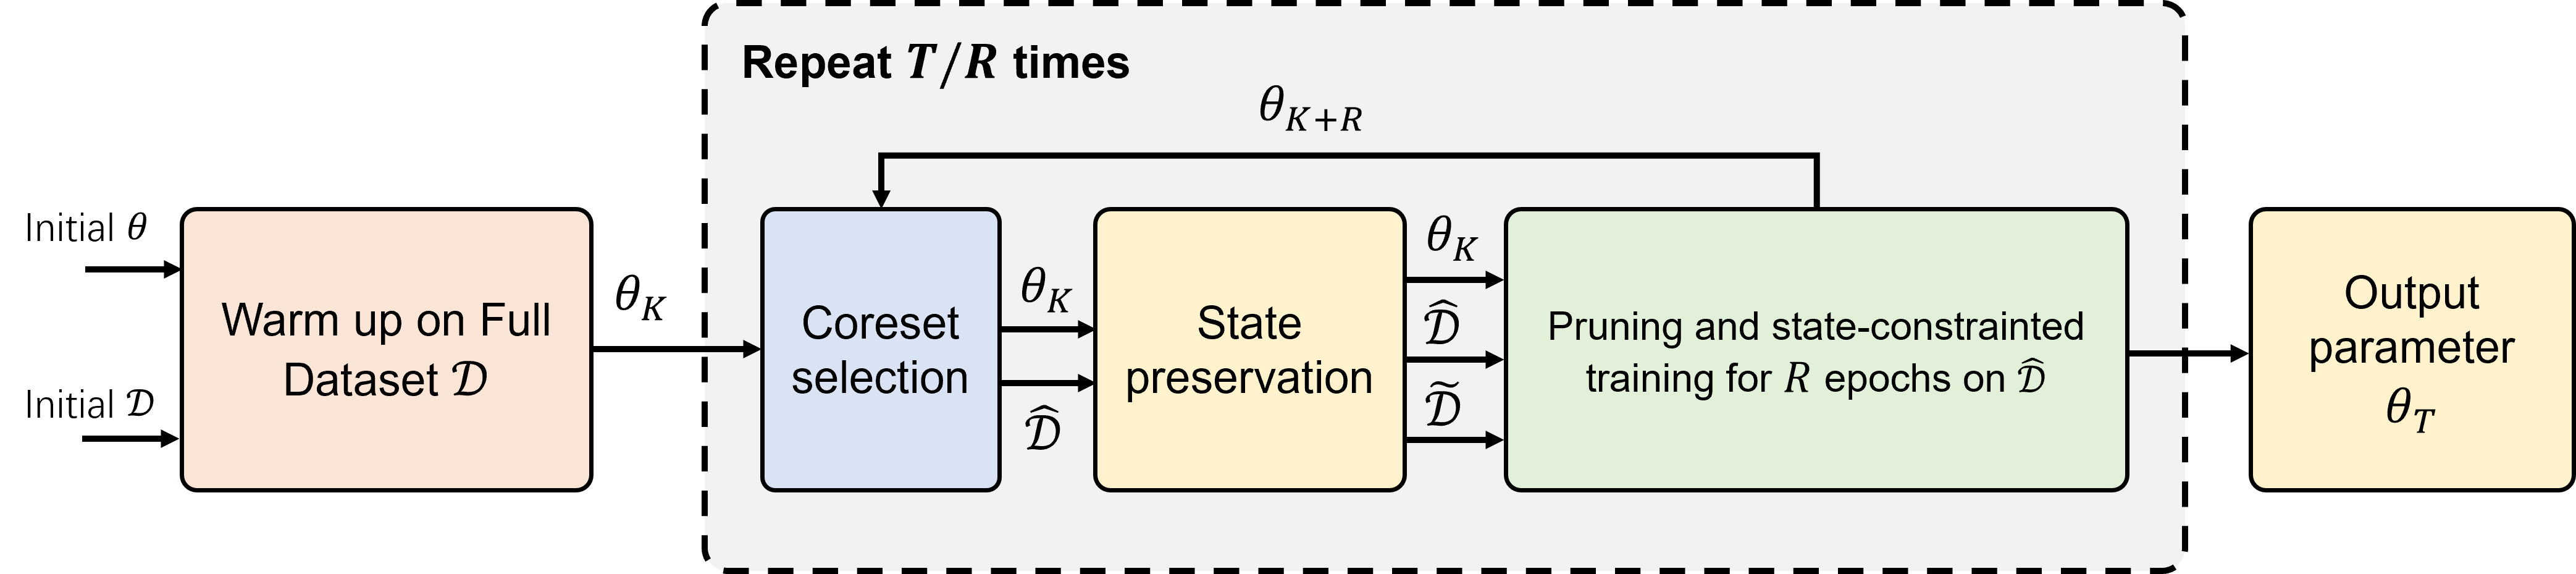
\includegraphics[width=0.75\linewidth]{figs/framework.png}
   \caption{Overview of SWaST, alternating between pruning and coreset selection every \(\mathcal{R}\) epochs. \(\mathcal{D}\) denotes the full dataset, \(\hat{\mathcal{D}}\) denotes the selected subset, \(\tilde{\mathcal{D}}\) denotes the stored logits, and \(T\) denotes the total epochs.}
   \label{fig:mechanism}
\end{figure*}

